\documentclass[english, 11pt]{article}
\usepackage{../../notes}
\usepackage{lipsum}

%Global Course Variables
\newcommand{\myCourseCode}{EECS 280}
\newcommand{\myCourseName}{Programming and Introductory Data Structures}
\newcommand{\myProf}{DeOrio, Juett, Mihalcea, \& Olson}
\newcommand{\myTerm}{Fall 2015}
\newcommand{\myLogo}{../um_seal.png}

%Headers
\lhead{\myCourseName}
\rhead{\fancyplain{}{\rightmark}} 

%Footers
\cfoot{\thepage}

\begin{document}
\titleHeader{\myCourseCode}{\myCourseName}{\myProf}{\myTerm}{\myLogo}

%Document information
\noindent\rule{1\columnwidth}{.5pt}
Contributors: Max Smith
\begin{center}
	Latest revision: \today
\end{center}
\toc
\abstr{Techniques and algorithm development and effective programming, top-down analysis, structured programming, testing, and program correctness. Program language syntax and static and runtime semantics. Scope, procedure instantiation, recursion, abstract data types, and parameter passing methods. Structured data types, pointers, linked data structures, stacks, queues, arrays, records, and trees.}

%----------------------------
%Document Begins
%----------------------------

\section{Introduction}
	\begin{itemize}
	\item See the syllabus.
\end{itemize}

\section{Procedural Abstraction and Recursion}
	\subsection{Notation}
\begin{itemize}
	\item $x\in\mathbb{R}^D$: data 
	\item $\phi (x)\in\mathbb{R}^M$: features for $\vec{x}$
	\item $t\in\mathbb{R}$: continuous-valued labels
	\item $\vec{x}^{(n)}\equiv \vec{x}_n$: n-th training example
	\item $\vec{t}^{(n)}\equiv \vec{t}_n$: n-th targe value
\end{itemize}

\subsection{1D Inputs}
\begin{itemize}
	\item In the 1D case ($x\in\mathbb{R}^1$)
	\item Given a set of observations $x^{(1)},\ldots ,x^{(N)}$ and corresponding targe values $t^{(1)},\ldots,t^{(N)}$
	\item We want to learn a function $y(\vec{x}, W)\approx t$ to predict future values
	$$y(\vec{x}, \vec{w})=\sum_{j=0}^{M-1}\vec{w}_j \phi_j (\vec{x}) = \vec{w}^T \phi(x)$$
	\item e.g., (green = solution, red = 3-rd polynomial approximation)
	\begin{center}
		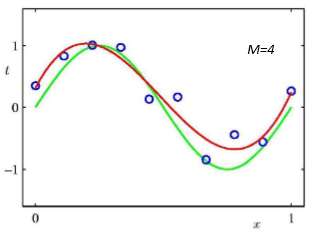
\includegraphics{sections/lec2/3.png}
	\end{center}
	\item For simplicity, we add a \textit{bias function}: $\phi_0 (\vec{x})=1$
	$$\vec{\phi}=1, x, x^2, x^3, \ldots$$
\end{itemize}

\subsection{Basis Function}
\begin{itemize}
	\item Function to construct features from raw data.
	\item e.g.,
	\begin{itemize}
		\item Polynomial: $\phi_j(x)=x^j$
		\item Gaussian: $\phi_j(x)=exp(-\frac{(x-\mu_j)^2}{2s^2})$
		\item Sigmoid: $\phi_j(x)=\sigma (\frac{x-\mu_j}{s})$
	\end{itemize}
\end{itemize}

\subsection{Objective Function}
\begin{itemize}
	\item We will use of sum-of-square errors:
	$$E(w)=\frac{1}{2}\sum_{n=1}^N (y(x^{(n)}, w)-t^{(n)})^2$$
\end{itemize}

\subsection{Batch Gradient Descent}
\begin{itemize}
	\item Given data $(x,y)$ initial $w$, repeat until convergence:
	$$\vec{w}=\vec{w}-\eta \nabla_{\vec{w}} E(\vec{w})$$
	$$\nabla_{\vec{w}}E(w)=\sum_{n=1}^N \left( \sum_{k=0}^{M-1} w_k \phi_k (\vec{x}^{(n)}) - t^{(n)} \right)\phi (\vec{x}^{(n)})=\sum_{n=1}^N \left(\vec{w}^T \phi (\vec{x}^{(n)}) - \vec{t}^{(n)}\right) \phi(x^{(n)})$$
\end{itemize}

\subsection{Overfitting}
\begin{itemize}
	\item An implicit way to tell is when the coeffecients become unreasonably large
	\item Solutions:
	\begin{itemize}
		\item Reduce order
		\item Add more data point
		\item Reselect features, some may be harming you
	\end{itemize}
	\item If you have a small number of data points, then you should use low order polynomial (small number of features)
	\item As you obtain more data points, you can gradually increase the order of the polynomial (more features)
	\item Controlling model complexity: \textbf{regularization}
\end{itemize}

\section{Tail Recursion}
	\subsection{Another kind of factorial}
\begin{lstlisting}[style=C++]
int fact_helper(intn, intresult){
	// REQUIRES: n >= 0
	// EFFECTS: returns result * n!

	if (n == 0) {
		return result;
	}else {
		return fact_helper(n-1,result*n);
	}
}

int factorial(intnum){
	// REQUIRES: num>= 0
	// EFFECTS: returns num!

	return fact_helper(num, 1);
}
\end{lstlisting}

\subsection{Stack effects}
\begin{itemize}
	\item Trace out the stack calls for \lstinline[style=C++]{factorial(2)} for our new and ``old'' function:
	\begin{center}
		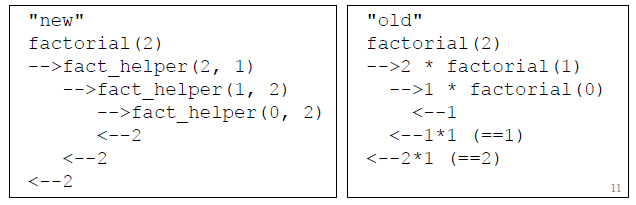
\includegraphics[scale=0.7]{sections/lec3/fact.png}	
	\end{center}

	\item Effects of the new version on the stack:
	\begin{itemize}
		\item The activation record of a function is needed only as long as there is computation left over and can be discarded as soon as the return value is known.
		\item With the new version, the concrete return value isn’t known at the time of the recursive call. However, we do know that whatever that recursive call returns, that will be our return value too.
		\item This means that the caller's stack frame isn't needed any more, and we can throw it away.
	\end{itemize}

	\item This is called \textbf{tail recursion}.
	\item If the result of the recursive call is returned directly with no pending computation, it is tail-recursive. Otherwise, it’s ``plain'' recursion.
\end{itemize}


\section{Recursion and Iteration}
	\subsection{Tail-recursion to iteration conversion}
\begin{itemize}
	\item There are five steps to the conversion of a tail-recursive function to an iterative one:
	\begin{enumerate}
		\item Copy the function's type signature
		\item Identify any needed ``loop variables'' by inspecting the call to the helper function (if it exists).
		\item Write initialization code to mirror the call to the helper function
		\item Identify termination condition(s) and return values by copying the base case behavior.
		\item Write loop body by copying the inductive step
	\end{enumerate}
\end{itemize}

\subsection{Dependency Graphs}
\begin{itemize}
	\item Special kind of graph with ``directed'' edges showing which ``new'' values depend on which ``old'' values.
	\item An edge is drawn from a \textbf{source vertex} to a \textbf{sink vertex}.
	\item To build a dependency graph, draw one vertex for each variable. If variable fooreads from variable barto compute its new value, draw an edge fromfootobar. (Don't draw an edge between a vertex and itself).
	\item If a variable has no edges with it as a sink(i.e. no edges terminate there), you can write its assignment, and erase it and any edges with it as a source.
	\item If two variables (\lstinline[style=C++]{foo, bar}) are each dependent on the other, then you can solve this by inventing shadow variables:
\begin{lstlisting}[style=C++]
int foo_new = bar - 1; // Shadow variable
int bar_new = foo - 1; // Shadow variable
// ------------------
foo = bar_new;
bar = foo_new;
\end{lstlisting}
	\item The transition between these two steps is called a \textbf{software epoch} - dependencies do not exist across epochs.
\end{itemize}

\section{Testing and Function Pointers}
	\subsection{After calibration}
\img{.8}{sections/lec5/p.png}
\begin{itemize}
	\item Internal parameters $K$ are known
	\item $R, T$ are known - but these can only relate $C$ to the calibraiton rig.
	\item You can't estimate $P_i$ from the single image measurement of $p_i$ because it may be anywhere along the line in space.
	\item We also don't have any information in the image to tell us the scale of anything in the world.
\end{itemize}

\subsection{Recovering structure from a single view}
\begin{itemize}
	\item You can make assumptions to get relative sizes of objects in images
	\item Pick a reference plane in the scene
	\item Pick a reference direction (not parallel to the reference plane) in the scene
	\img{.8}{sections/lec5/ref.png}
	\subsubsection{Geometry}
	\img{.8}{sections/lec5/van.png}
	\item Under perspective projection, parallel lines in three-space project to convering lines in the image plane. The common point of intersection, perhaps at infinity, is called the \textbf{vanishing point}
	\begin{itemize}
		\item projection of a point at infinity (goes infinity far)
		\img{.8}{sections/lec5/vp.png}
		\item Any two parallel lines have the same vanishing point
		\item The ray from $C$ through $v$ point is parallel to the lines
		\item AN image may have more than one vanishing point
	\end{itemize}
	\item Two or more vanishing points from lines known to lie in a single 3D plane establish a \textbf{vanishing line}, which completely determines the orientation of the plane
	\img{.7}{sections/lec5/house.png}
\end{itemize}

\subsection{The Cross Ratio}
\img{.8}{sections/lec5/y.png}
\begin{itemize}
	\item $Y$ is desired height to measure
	\item Compute Y from image measurements
	\begin{itemize}
		\item You'll need more than vanishing points to compute this
	\end{itemize}
	\item \textbf{Projective Invariant}: something that does not change under projective transformations (including perspective projection)
	\img{.8}{sections/lec5/l.png}
	\item The \textbf{cross ratio} of 4 collinear points is projective invariant
	$$\frac{||P_3 - P_1||\cdot ||P_4 - P_2||}{||P_3 - P_2||\cdot ||P_4 - P_1||}$$
	\item You can permute the point ordering and it will remain true.
	\item Often called the fundamental invariant of projective geometry
	\img{.8}{sections/lec5/inf.png}
	\item When you consider the points at $\infty$, and the point where the camera would meet the ground plane $v_z$ you have enough points to use the cross ratio on our camera model.
	\item You need the same points in the world and camera system (can't mix and match)
	\item You must make some assumption to determine the relative sizes, typically assume $L$
\end{itemize}

\subsection{Horizon line}
\img{.7}{sections/lec5/hor.png}
\begin{itemize}
	\item Sets of parallel lines on the same plane lead to collinear vanishing points the line is called the \textbf{horizon}
	\img{.8}{sections/lec5/ex.png}
	\item When trying to recover the structure within the camera reference system, we can check if two linesare parallel or not
	\begin{itemize}
		\item If they do, recognize the horizon line
		\item Measure if hte 2 lines meet the horizon
		\item If they do, they are parallel in 3D
		\item Actual scale of scene is not recovered, only relative distances
	\end{itemize}
\end{itemize}

\subsection{Lines in a 2D plane}
$$ax+by+c=0; l=\begin{bmatrix}
	a\\b\\c
\end{bmatrix}$$
\subsubsection{Intersecting lines}
\img{1}{sections/lec5/intersect.png}
\begin{itemize}
	\item The intersection of lines can be calculated with: 
	$$x=l\times l'$$
\end{itemize}

\subsection{Stereo-view geometry}
\img{1}{sections/lec5/tri.png}
\begin{itemize}
	\item Two camera perspectives allow us to find position of objects through \textbf{triangulation}
	\begin{itemize}
		\item This requires a few knowns, $K_1, K_2, R, T$
	\end{itemize}
	\item Small inaccuracies with knowns can lead to situations where the lines may not intersect 
	\item Instead, we'll find where they came close enough
		$$d^2(x_1, M_1X)+d^2(x_2, M_2X)$$
		$$d:=\text{distance between two lines}$$
\end{itemize}

\subsection{Epipolar Geometry}
\img{.7}{sections/lec5/ep.png}
\begin{itemize}
	\item \textbf{Epipolar plane} (grey): intersections of baseline with image planes
	\item \textbf{Baseline} (orange): projectison of other camera center
	\item \textbf{Epipolar lines} (blue): vanishing points of camera motion direction
	\item This framepoint, allows us to consider if two pointsare related by epipolar geometry
	\item Use epipolar lines to find sharing points will greatly save computation cost as a 2D search becomes 1D
	\subsubsection{Parallel image planes}
	\item Baseline intersects the image plane at infinity
	\item Epipoles are at infinity
	\item Epipolar lines are parallel to x-axis
	\subsubsection{Forward translation}
	\img{1}{sections/lec5/f.png}
	\item When a camera moves forward the lines turn into a spiral
\end{itemize}

\section{Arrays and Pointers}
	\subsection{Recap - Bounds Checking for Arrays Example}
\subsubsection{Basic Layout}
\begin{lstlisting}[style=C++]
class Array {
 public:
    Array(unsigned len = 0) : length(len) {
        data = (len ? new double[len] : nullptr);
    }
 private:
    double *data;        // array data
    unsigned int length; // array size
}
\end{lstlisting}
You could use a struct, but users of your class would be able to access all member variables of your struct by default.

\subsubsection{Copy Constructor}
To copy the array, you need to perform a \textit{deep copy}:
\begin{lstlisting}[style=C++]
Array(const Array & a) {
    length = a.getLength(); // getter for length // 1 step
    data = new double[length];                   // 1 step
    for (unsigned i = 0; i < length; i++) {      // n times
        data[i] = a[i];                          // c steps
    }
}
\end{lstlisting}
The complexity of this is: $\O{! + 1 + (nc) + 1}=\O{n}$

\subsubsection{Better Copying}
\begin{lstlisting}[style=C++]
void copyFrom(const Array & a) {
    if (length != a.length) {
        delete[] data;
        length = a.length;
        data = new double[length];
    }

    for (unsigned int i = 0; i < length; i++) {
        data[i] = a.data[i];
    }
}

Array(const Array & a) : length(0), data(nullptr) {
    copyFrom(a);
}

Array & operator=(const Array & a) {
    copyFrom(a);
    return *this;
}
\end{lstlisting}

\subsection{The Big 5}
\begin{itemize}
	\item Destructor
	\item Copy constructor
	\item Overloaded operator=
	\item Copy constructor from \textit{r-value}
	\item Overloaded operator= from \textit{r-value}
\end{itemize}

\subsubsection{Destructor}
\begin{lstlisting}[style=C++]
~Array() {
    if (data != nullptr) {
        for (int i = 0; i < length; i++) { // n times
            delete data[i];                // 1 step
        }
        delete[] date;                     // 1 step
        data = nullptr;                    // 1 step
    }
}
\end{lstlisting}
Complexity: $\O{n}$

\subsubsection{Access Operator[]}
\begin{lstlisting}[style=C++]
const double & operator[](int idx) const {
    if (idx < length && idx >= 0)
        return data[idx];
    throw runtime_error("bad idx");
}
\end{lstlisting}
\begin{itemize}
	\item Declares read-only access/
	\item Automatically selected by the compiler when an array being access is marked \lstinline[style=C++]{const}
	\item Helps compiler optimize code for speed
	\item Some functions, like \lstinline[style=C++]{ostream &operator<<(ostream &os, const Array &a)} require \lstinline[style=C++]{const}.
	\item Must also make a non-constr version
\end{itemize}

\subsubsection{Access with more than 2 dimensions}
\begin{lstlisting}[style=C++]
const double &operator()(int i, int j) const {
    // return by const reference
}
\end{lstlisting}
\begin{itemize}
	\item Can't overload \lstinline[style=C++]{operator[][]}
\end{itemize}

\subsubsection{Inserting an Element}
\begin{lstlisting}[style=C++]
bool insert(int index, double val) {
    if (index >= size || index < 0) {
        return false;
    } else {
        for (int i = size - 1; i > index; --i) {
            data[i] = data[i - 1];
        }
        data[index] = val;
        return true;
    }
}
\end{lstlisting}
Complexity:
\begin{itemize}
	\item Best case: $\O{1}$
	\begin{itemize}
		\item The element is inserted at the end
	\end{itemize}

	\item Average case: $\O{n}$
	\begin{itemize}
		\item Go through half of elements (but that is a constant times $n$)
	\end{itemize}

	\item Worst case: $\O{n}$
	\begin{itemize}
		\item Go through all elements
	\end{itemize}
\end{itemize}

\subsubsection{Append}
When array is full, resize:
\begin{itemize}
	\item Double array size from $n$ to $2n$
	\item Copy $n$ items from the original array to the new array
	\item Appending $n$ elements
	\item Total: $1 + n + n = 2n + 1$ steps
	\item Amortized: $(2n+1)/n=\O{1}$ steps
\end{itemize}

\subsection{Linked Lists and Iterators}
\begin{itemize}
	\item \textbf{Linked list}: Each person points to the next person
	\item \textbf{Doubly linked list}: Each person points to each other
	\item \textbf{Circularly linked list}: A list which has the first and last nodes pointing to each other
\end{itemize}

\subsubsection{Arrays vs Linked Lists}
Arrays:
\begin{itemize}
	\item Access:
	\begin{itemize}
		\item Random: $\O{1}$ time
		\item Sequential: $\O{1}$ time
	\end{itemize}

	\item Insert:
	\begin{itemize}
		\item Insert: $\O{n}$ time
		\item Append: $\O{n}$ time
	\end{itemize}

	\item Book-keeping:
	\begin{itemize}
		\item \lstinline[style=C++]{ptr} to beginning
		\item \lstinline[style=C++]{current_size} or \lstinline[style=C++]{ptr}
		\item \lstinline[style=C++]{max_size} or \lstinline[style=C++]{ptr} to end off allocated space
	\end{itemize}

	\item Memory:
	\begin{itemize}
		\item Wastes memory if size is too large
		\item Requires reallocation if too small
	\end{itemize}
\end{itemize}
Linked Lists:
\begin{itemize}
	\item Access:
	\begin{itemize}
		\item Random: $\O{n}$ time
		\item Sequential: $\O{1}$ time
	\end{itemize}

	\item Insert:
	\begin{itemize}
		\item Insert: $\O{n}$ time
		\item Append: $\O{1}$ time
		\begin{itemize}
			\item Append to \lstinline[style=C++]{tail_ptr}
		\end{itemize}
	\end{itemize}

	\item Book-keeping:
	\begin{itemize}
		\item \lstinline[style=C++]{head_ptr} to first node
		\item \lstinline[style=C++]{size} (optional)
		\item \lstinline[style=C++]{tail_ptr} to last node
		\item In each node, \lstinline[style=C++]{ptr} to next node
		\item Wasteful for small data times (overhead on pointers)
	\end{itemize}

	\item Memory:
	\begin{itemize}
		\item Allocates memory as needed
		\item Requires memory for pointers
	\end{itemize}
\end{itemize}

\subsection{Linked List Implementation}
\begin{lstlisting}[style=C++]
class LinkedList {
 public:
    LinkedList();
    ~LinkedList();
 private:
    struct Node {
        double item;
        Node *next;
        Node() {next = nullptr;}
    };

    Node *head_ptr;
};
\end{lstlisting}

\subsubsection{Methods}
\begin{lstlisting}[style=C++]
int size() const;

bool append_item(double item);
bool append_node(Node *n);

bool delete_item(double item);
bool delete_node(Node *n);
\end{lstlisting}

\subsubsection{Maintaining Consistency}
Arrays:
\begin{itemize}
	\item Stored size matches number of elements at all times
	\item Be sure that \lstinline[style=C++]{start_ptr + size < end_ptr}
\end{itemize}
Linked Lists
\begin{itemize}
	\item Stored size matches number of elements
	\item The last node points to \lstinline[style=C++]{nullptr}
	\item If the list is a circular list, last node points to head
	\item If a doubly-linked list, next/prev pointers are consistent
\end{itemize}

\section{Array Traversal}
	\subsection{Passing Pointers to Functions}
\begin{itemize}
	\item Pointers can be arguments to functions. For example, suppose you want a function that adds one to an integer argument passed by reference:
\begin{lstlisting}[style=C++]
void add_one(int *x){
	// MODIFIES: *x
	// EFFECTS: adds one to *x
	*x = *x + 1;
}
\end{lstlisting}
	\item If you were to call this function as so: \lstinline[style=C++]{add_one(bar);}, where \lstinline[style=C++]{bar} is a pointer to \lstinline[style=C++]{foo}
\begin{lstlisting}[style=C++]
int foo;
int *bar;
bar = &foo;

add_one(bar);
\end{lstlisting}
	\begin{itemize}
		\item The variable bar is bassed by \textbf{value}, but it's a pointer!
		\item Both bar and the copy of bar refer to the same address in memory.
	\end{itemize}
	\item You can also make the call without the ``middleman'' like: \lstinline[style=C++]{add_one(&foo);}
\end{itemize}

\subsection{Pointer question}
\begin{itemize}
	\item If you modify \lstinline[style=C++]{add_one} to:
\begin{lstlisting}[style=C++]
void add_one(int *x){
	x = x + 1;
}
\end{lstlisting}	
	\item It will increment the value \textbf{of the pointer} by one.
	\item Pointer arithmetic is done based on units of the \textbf{referent type} (the type of the objects in the list).
\end{itemize}

\subsection{Pointers vs. references}
\begin{itemize}
	\item Both allow you to pass objects by reference.
	\item Pointers require some extra syntax at calling time (\&), in the argument list (*), and with each use (*); references only require extra syntax in the argument list (\&).
	\item You can change the object to which a pointer points using arithmetic/assignment, but you cannot change the object to which a reference refers.
	\item You might wonder why you’d ever want to use pointers, since theyrequire extra typing, and allow you to shoot yourself in the foot.
	\item Why use pointers?
	\begin{itemize}
		\item Array variables are internally implemented using pointers
		\item They allow us to create structures (unlike arrays) whose size is not known in advance; we won't see that use until the last third of the course.
	\end{itemize}
\end{itemize}

\subsection{Pointers and Arrays}
\begin{itemize}
	\item Arrays are actually represented via pointers as so:
	\begin{center}
		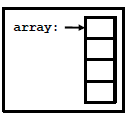
\includegraphics{sections/lec7/array.png}
	\end{center}
	\item If you were to look at the value of the variable ``array'' (not \lstinline[style=C++]{array[0]}) you'd find that it was exactly the same as the address of \lstinline[style=C++]{array[0]}.
	\item When the argument \lstinline[style=C++]{array} is passed to the function sum, a pointer to the first element of the array is really passed and the compiler does all the work of translating something like: \lstinline[style=C++]{array[3]} into the proper arithmetic/dereference to get the right value.
\begin{lstlisting}[style=C++]
x = array[3];
// Is equivalent to:
int *tmp;
tmp = array + 3;
x = *tmp;
// Or simply:
x = *(array + 3);
\end{lstlisting}
\end{itemize}

\subsection{Indexing vs. pointer arithmetic}
\begin{itemize}
	\item Using array indexing:
\begin{lstlisting}[style=C++]
for (int i = 0; i < SIZE; ++i){
	cout << array[i] << " ";
}
\end{lstlisting}
	\item Using pointer arithmetic:
\begin{lstlisting}[style=C++]
for (int *i = array; i < array+SIZE; ++i){
	cout << *i << " ";
}
\end{lstlisting}
\end{itemize}

\subsection{Array Traversal Using Pointers}
\begin{lstlisting}[style=C++]
int strlen(char *s) {
	char *p = s;
	while (*p) ++p;
	return p - s;
}
\end{lstlisting}
\begin{itemize}
	\item \lstinline[style=C++]{*p} evalues to ``false'' if \lstinline[style=C++]{p} points to a NULL, true otherwise.
	\item \lstinline[style=C++]{++p} advances by ``one character''
	\item \lstinline[style=C++]{p-s} computes the ``number of characters'' between \lstinline[style=C++]{p} and \lstinline[style=C++]{s}
\end{itemize}

\subsection{Constants}
\begin{itemize}
	\item \lstinline[style=C++]{void strcpy(char *dest, const char *src);}
	\item \lstinline[style=C++]{const} is a \textbf{type qualifier} - something that modifies a type
	\item It means ``you cannot change this value once you have initialized it.''
	\item When you have pointers, there are two things you might change:
	\begin{itemize}
		\item The value of the pointer.
		\item The value of the object to which the pointer points.
	\end{itemize}
	\item Either (or both) can be made unchangeable:
\begin{lstlisting}[style=C++]
const T *p;			// "T" (the pointed-to object) cannot be changed
T *const p;			// "p" (the pointer) cannot be changed
const T *const p;	// neither can be changed.
\end{lstlisting}
	\item Adding \lstinline[style=C++]{const} will stop changing value mistakes, and the compiler will catch them.
	\item You can use a pointer-to-T anywhere you expect a pointer-to-const-T, but NOT vice versa
	\item That's because code that expects a pointer-to-T might try to change the T, but this is illegal for a pointer-to-const-T.
	\item However, code that expects a pointer-to-const-T will work perfectly well for a pointer-to-T; it's just guaranteed not to try to change it.
\end{itemize}

\subsection{C strings vs. C++ strings}
\begin{center}
\begin{tabular}[breaklines=true]{p{5cm}|p{5cm}|p{5cm}}
	& C string & C++ string \\
	\hline
	Library headers & 
{\begin{lstlisting}[style=C++] 
#include <string>
\end{lstlisting}} & 
{\begin{lstlisting}[style=C++]
#include string
\end{lstlisting}}\\	
	string constant &
{\begin{lstlisting}[style=C++]
constchar* hello = "hello";
\end{lstlisting}}&
{\begin{lstlisting}[style=C++]
conststring hello = "hello";
\end{lstlisting}} \\
	length &
{\begin{lstlisting}[style=C++]
strlen(hello);//5
\end{lstlisting}} &
{\begin{lstlisting}[style=C++]
hello.length();//5
\end{lstlisting}} \\
	local variable &
{\begin{lstlisting}[style=C++]
constintMAXSIZE=1024; 
char s[MAXSIZE];
\end{lstlisting}} &
{\begin{lstlisting}[style=C++]
string s;
\end{lstlisting}} \\
	copy &
{\begin{lstlisting}[style=C++]
strcpy(s, hello);
\end{lstlisting}} &
{\begin{lstlisting}[style=C++]
s = hello;
\end{lstlisting}} \\
	concatenate &
{\begin{lstlisting}[style=C++]
constchar* world = " world";
char message[MAXSIZE];
strcpy(message, hello);
strcat(message, world);
\end{lstlisting}} &
{\begin{lstlisting}[style=C++]
string message = hello + " world";
\end{lstlisting}} \\
	compare &
{\begin{lstlisting}[style=C++]
if (strcmp(a,b) == 0)
	// do something
\end{lstlisting}} &
{\begin{lstlisting}[style=C++]
if (a == b)
	// do something
\end{lstlisting}} \\
	convert to C++ string &
{\begin{lstlisting}[style=C++]
string cpp_str = hello;
\end{lstlisting}} &
{\begin{lstlisting}[style=C++]
char c_str[MAXSIZE];
strcpy(c_str, message.c_str());
\end{lstlisting}} \\
\end{tabular}
\end{center}

\subsection{Type Sizes}
\begin{itemize}
	\item The amount of memory assigned to a data type is a source of innumerable ``portability bugs'' in programs.
	\item There are \textbf{some} guarantees, however:
	\begin{itemize}
		\item A ``char'' is always one byte
		\item A ``short'' is always at least as big as a char
		\item An ``int'' is always at least as big as a short
		\item A ``long'' is always at least as big as an int
	\end{itemize}
	\item \lstinline[style=C++]{sizeof(int)} tells you the number of bytes required to store an \lstinline[style=C++]{int}
	\begin{center}
		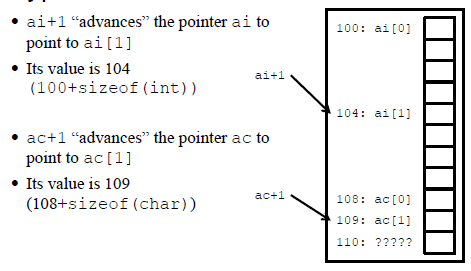
\includegraphics{sections/lec7/type.png}
	\end{center}
\end{itemize}

\section{Argv, IO, Enums, and Templates}
	\subsection{Argv Basics}
\begin{itemize}
	\item Arguments are passed to programs as an array too \lstinline[style=C++]{int main(intargc, char *argv[])}
	\item Since each argument is just a sequence of characters, this array is an array of C-strings: \lstinline[style=C++]{char *argv[]}
	\begin{center}
		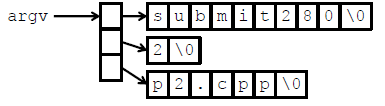
\includegraphics{sections/lec8/argv.png}
	\end{center}
	\item We also need to know how big the array is: \lstinline[style=C++]{int argc}
	\item Suppose we wanted to write a program that is given a list of integers as it’s arguments, and prints out the sum of that list (you'll need to convert the strings to int):
\begin{lstlisting}[style=C++]
intatoi(const char *s);
// EFFECTS: parses s as a number and returns its int value
\end{lstlisting}
\end{itemize}

\subsection{Shell Redirection}
\begin{itemize}
	\item Redirect a file to our program's standard input (cin): \lstinline[style=bash]{./a.out < inputfile>}
	\item Redirect our programs' standard output (cout) to a file: \lstinline[style=bash]{./a.out > outputfile}
	\item This is not File IO, that is done directly instead of the shell.
\end{itemize}

\subsection{File IO}
\begin{lstlisting}[style=C++]
// Open a file using a filestream
string filename = "hello.txt";
ifstreamfilestream;
filestream.open( filename.c_str() );

// CHeck for success opening file
if ( !filestream.is_open() ) {
	cour<< "open failed" << endl;
	exit(1);
}

// Read one word at a time and check that the read was successful
string word;
while ( filestream >> word ) {
	cout<< "word = `" << word << "'\n";
}

// Close file after reading is finished
filestream.close();

/* Alternative: read two words at a time
	string word1, word2;
	while ( filestream>> word1 >> word2 ){
		cout << "word1 = `" << word1 << "'\n"
			 << "word2 = `" << word2 << "'\n";
	}
 */

/* Alternative: read numbers
	int i;
	while (filestream >> i) {
		cout << "i = " << i << endl;
	}
 */
\end{lstlisting}

\subsection{Enums}
\begin{itemize}
	\item Enumeration allows for the categorizing of data
\begin{lstlisting}[style=C++]
enum Month {JAN, FEB, MAR, APR, MAY, JUN,
			JUL, AUG, SEP, OCT, NOV, DEC};
enum Semester {WINTER, SPRING, SUMMER, FALL};

// Define a variable of the new type:
Month this_month;
Semester this_semester;

// Initialize your variables:
this_month = MAY;
this_semester = SPRING;
\end{lstlisting}
	\item Once you have an \lstinline[style=C++]{enum} type defined, you can use it as a function input or output, just like any other type
	\item \lstinline[style=C++]{enum} types are passed by value by default
\end{itemize}

\subsection{Switch statements}
\begin{itemize}
	\item Switch statements work well with enums, and are much faster than long chains of if/else/if/else statements
	\item Two cases with the same result are grouped together since the arms of the case statement ``fall through'' to the next \lstinline[style=C++]{break}
\begin{lstlisting}[style=C++]
Semester s = FALL;
switch(s) {
	case SPRING:
	case SUMMER:
		cout<< "vacation!\n";
		break;
	case FALL:
	case WINTER:
		cout<< "work!\n";
		break;
	default:  // Add a default, just in case
		assert(0); // error!
		exit(1);
}
\end{lstlisting}
\end{itemize}

\subsection{Templates}
\begin{itemize}
	\item The intuition behind templates are that they are code with the ``type name'' left as a (compile-time) constant.
	\item The basic idea of templates is that you declare something to be a template, parameterized across one or more types: \lstinline[style=C++]{template <typename T>}
	\item Then, write the definition of the function you want templated, using the type \lstinline[style=C++]{T} where appropriate:
\begin{lstlisting}[style=C++]
template <typenameT>
	T sum(T a[], intsize) {
	//REQUIRES: T can be initialized to 0 and “+”
	//is defined over T.
	T result = 0;
	for (int i = 0; i<size; ++i)
		result += a[i];
	return result;
}
\end{lstlisting}
	\item Now, we can use this single definition to serve the purposes of both of the ``old'' functions:
\begin{lstlisting}[style=C++]
double a[100] = {... }
intb[200] = {... }
intc[100] = {... }

double aSum= sum(a, 100);
intbSum= sum(b, 200);
intcSum= sum(c, 100);
\end{lstlisting}
	\item How it works:
	\begin{enumerate}
		\item When the compiler sees the first call to \lstinline[style=C++]{sum()}, it inspects the type of the first argument, because that's the ``template type''.
		\item It then generates the code for that version of \lstinline[style=C++]{sum()}, substituting the word \lstinline[style=C++]{double} for the type variable \lstinline[style=C++]{T}. This is called ``instantiation''.
		\item When it sees the second call to \lstinline[style=C++]{sum()}, it does the same thing by generating a second version of \lstinline[style=C++]{sum()} and substituting the word \lstinline[style=C++]{int} for the type variable \lstinline[style=C++]{T}.
		\item When it sees the third call, the compiler knows that that variant of \lstinline[style=C++]{sum()} already exists and simply reuses it.
	\end{enumerate}
\end{itemize}

\section{Structs and Classes}
	\subsection{Structs}
\begin{itemize}
	\item A \lstinline[style=C++]{struct} describes a ``compound object'' that comprises one or more elements, each of independent type
	\item Defines a new type, containing only data
	\item e.g., a triangle:
\begin{lstlisting}[style=C++]
struct Triangle {
	double a, b, c; // Edge lengths
}

int main() {
	Triangle t; // New triangle with undefined edges

	// Initialize each member
	t.a = 3;
	t.b = 4;
	t.c = 5;

	// Or initialize member variables all at once, in order:
	Triangle t2 = {3, 4, 5};

	// Copy
	Triangle t3 = t2;
}
\end{lstlisting}
	\item \lstinline[style=C++]{struct} are passed by value, unlike arrays
	\item This can be a problem with large structs, so pass by reference or pointer
\end{itemize}

\subsection{struct vs. array}
\begin{center}
\begin{tabular}[breaklines=true]{p{5cm}|p{5cm}}
	struct & array \\
	\hline
	{\begin{lstlisting}[style=C++]
struct Triangle{/*...*/};
	 	\end{lstlisting}} &
	{\begin{lstlisting}[style=C++]
double edges[3];
	 	\end{lstlisting}} \\
	Stores group of data & Stores group of data \\
	Heterogeneous types & Homogenous types \\
	Access by name & Acces by index \\
	Default pass-by-value & Default pass-by-reference \\
	Creates a custom type & Does not create a new type \\
\end{tabular}
\end{center}

\subsection{struct vs. class}
\begin{center}
\begin{tabular}{l|l}
	struct & class \\
	Heterogeneous aggregate data type & Heterogeneous aggregate data type \\
	C style & C++ style \\
	Contains only data & Contains data and functions \\
	Undefined by default & Constructors can be used to initialize \\
	All data is accessible & Control of data access \\
\end{tabular}
\end{center}

\subsection{Classes}
\begin{itemize}
\begin{lstlisting}[style=C++]
class Triangle {
	public:
	double a,b,c;//edge lengths

	double area(){ //compute area
		double s = (a+b+c)/2;
		double newArea= sqrt(s*(s-a)*(s-b)*(s-c));
		return newArea;
	}
};
\end{lstlisting}
	\item A \lstinline[style=C++]{class} contains both data and functions
	\item These are called \textbf{member data} and \textbf{member functions}
	\item Because member functions are within the same scope as member data, they have access to the member data directly
	\item \lstinline[style=C++]{public} means members are accessible from outside the \lstinline[style=C++]{class}
	\item From outside scope, access \lstinline[style=C++]{class} members just like a \lstinline[style=C++]{struct}
\begin{lstlisting}[style=C++]
int main() {
	Triangle t;
	t.a=3; t.b=4; t.c=5;
	cout << "area = " << t.area() << endl;

	// Copy
	Triangle t2 = t1;
}
\end{lstlisting}
	\item Calling a member function is just like evaluating a function
\end{itemize}

\subsection{Initialization problem}
\begin{itemize}
	\item Classes, similar to structs, has undefined values upon initialization.
	\item This is a common source of bugs.
	\item A \textbf{constructor} is a member function that has the same name as the class
	\item They run automatically when a new object is defined
	\item It's typically used to initialize member variables
	\item A constructor has the same name as the class, and no return value:
\begin{lstlisting}[style=C++]
class Triangle {
public:
	double a, b, c;
	double area() {/*...*/}

	// Constructor
	Triangle() {a=0; b=0; c=0;}

	// Constructors with inputs for initialization 
	Triangle(double a_in, double b_in, double c_in){
		a = a_in; b = b_in; c = c_in;
	}
}

int main() {
	Triangle t; // Constructor executes automatically
	t.area();
}
\end{lstlisting}
	\item The compiler will select the correct constructor
	\item Two different functions with the same name, but different prototypes is called \textbf{function overloading}.
	\item There are several ways to call the initializer:
\begin{lstlisting}[style=C++]
int main() {
	Triangle t = Triangle(3, 4, 5);
	Triangle t2(3, 4, 5);
}
\end{lstlisting}
\end{itemize}

\subsection{Private member variables}
\begin{itemize}
	\item Declaring variables and functions as \lstinline[style=C++]{private} allows them to be only visible within the scope of that respective class.
\begin{lstlisting}[style=C++]
class Triangle {
private:
	double a, b, c;
public:
	//...
}
\end{lstlisting}
	\item In this example, calling \lstinline[style=C++]{t.a} is no longer possible.
	\item By default, every member of a class is \lstinline[style=C++]{private}
\end{itemize}

\subsection{get and set functions}
\begin{itemize}
	\item A \lstinline[style=C++]{get} function is a \lstinline[style=C++]{public} function that returns a copy of a \lstinline[style=C++]{private} member variable:
\begin{lstlisting}[style=C++]
class Triangle {
	//...
public: 
	// EFFECTS: returns edge a, b, c
	double get_a() {return a; }
	double get_b() {return b; }
	double get_c() {return c; }
}
\end{lstlisting}
	\item A \lstinline[style=C++]{set} function is a \lstinline[style=C++]{public} function that modifies a \lstinline[style=C++]{private} member variable:
\begin{lstlisting}[style=C++]
class Triangle {
	//...
public: 
	// REQUIRES: a,b,care non-negative and form a triangle
	// MODIFIES: a, b, c
	// EFFECTS: sets length of edge a, b, c
	void set_a(double a_in);
	void set_b(double b_in);
	void set_c(double c_in);
}
\end{lstlisting}
	\item \lstinline[style=C++]{set} functions allow you to run extra code when a member variable changes
\end{itemize}

\subsection{struct vs. class}
\begin{center}
\begin{tabular}{l|l}
	struct & class \\
	\hline
	Heterogeneous aggregate data type & Heterogeneous aggregate data type \\
	C style & C++ style \\
	Contains only data & Contains data and functions \\
	Undefined by default & Constructs can be used to initialize \\
	All data is accessible & Control of data access \\
\end{tabular}
\end{center}

\section{Abstract Data Types (ADTs)}
	\subsection{Abstraction}
\begin{itemize}
	\item \textbf{Procedural abstraction}
	\begin{itemize}
		\item A function is given a specification which documents whatthe function does, but not howit does it.
		\item For example, if we find a faster way to compute factorial, we can just replace the old implementation with the new one, and no other component of the program needs to know this.
	\end{itemize}
	\item \textbf{Data abstraction}
	\begin{itemize}
		\item An ADT provides an abstractdescription of values and operations.
		\item The definition of an ADT must combine bothsome notion ofwhatthe values of that type represent, and howthey behave.
		\item We can leave off the details of how this actually happens.
	\end{itemize}
\end{itemize}

\subsection{Abstract Data Types}
\begin{itemize}
	\item \textbf{Information hiding}: we don't need to know the details of how the object is represented, nor do we need to know how the operations on those objects are implemented.
	\item \textbf{Encapsulation}: the objects and their operations are defined in the same place; the ADT combines both data and operation in one entity.
	\item ADTs are substitutable: you can change the implementation and no users of the type can tell
	\item See example in lecture slides.
\end{itemize}

\subsection{const member functions}
\begin{itemize}
	\item You can use \lstinline[style=C++]{const} in a function signature promises ``this member function will not modify any member variable''
\begin{lstlisting}[style=C++]
class Triangle {
	//...
	double area() const;
	//...
}
\end{lstlisting}
\end{itemize}

\subsection{Representation invariant}
\begin{itemize}
	\item Member variables are a class’s representation
	\item The description of how member variables should behave are representation invariants
	\item \textbf{Representation invariants} are rules that the representation must obey immediately before and immediately after any member function execution
	\item The \textit{what} the data type does is then the header file
	\item The \textit{how} the data type works is in the cpp file
\end{itemize}

\subsection{Scope Resolution Operator}
\begin{itemize}
	\item \lstinline[style=C++]{::} is the scope resolution operator, which tells the compiler that this function is inside the scope of the class
	\item e.g.,
\begin{lstlisting}[style=C++]
Triangle::Triangle(): a(0), b(0), c(0) {}
\end{lstlisting}
	\item In the previous example, it's used to show in-line construction
	\item This syntax is called an \textbf{initializer list}
	\item More efficient, because dealt with at compile time.
	\item It can also be used with parameters. e.g.,
\begin{lstlisting}[style=C++]
Triangle::Triangle(double a_in, double b_in, double c_in): a(a_in), b(b_in), c(c_in) {}
\end{lstlisting}
	\item See the Flatland example from lecture slides.
\end{itemize}

\section{Subtypes and Subclasses}
	\subsection{Hopfield Nets}
\begin{itemize}
	\item A hopfield net is composed of binary threshold units with recurrent connections between them
	\item Recurrent networks of non-linear units are generally very hard to analyze. THey can behave in many different ways:
	\begin{itemize}
		\item Settle to a stable state
		\item Oscillate
		\item Chaotic trajectories (cannot predict future)
	\end{itemize}

	\item John Hopfield realized that if the connections are symmetric, there is a global every function
	\begin{itemize}
		\item Each binary ``configuration'' of the whole network has an energy
		\item The binary threshold decision rule causes the network to a minimum of this energy function
	\end{itemize}

	\subsubsection{The energy function}
	\item The global energy is the sum of many contributions. Each contribution depends on one connection weight and the binary states of two neurons:
		$$E=-\sum_i s_i b_i - \sum_{i<j} s_i s_j w_{ij}$$
	\item This simple quadratic energy function makes it possible for each unit to compute locally how it's state affects the global energy:
		$$\text{Energy gap}=\delta E_i = E(s_i = 0) - E(s_i = 1) = b_i + \sum_j s_j w_{ij}$$
	\item Energy gap is the difference in energy when it is off minus when it is on
	
	\subsubsection{Settling to an energy minimum}
	\item To find an energy minimum in this net, start from a random state and then update units one at a time in random order
	\begin{itemize}
		\item Update each unit to whichever of its two states give the lowest global energy
		\item i.e., use binary threshold units
	\end{itemize}
	\begin{cetner}
		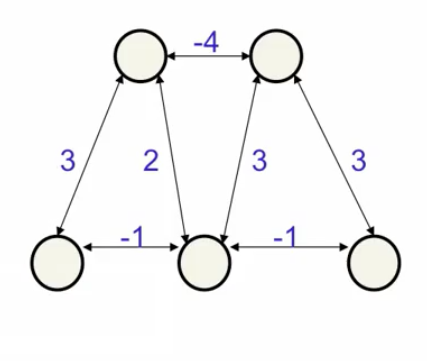
\includegraphics[scale=0.8]{sections/11/min.png}
	\end{cetner}
	$$-\text{Energy}=\text{goodness}=3$$

	\item A random unit is selected, and the question is asked: What state should that be in, given the current states of all other units?
	\begin{center}
		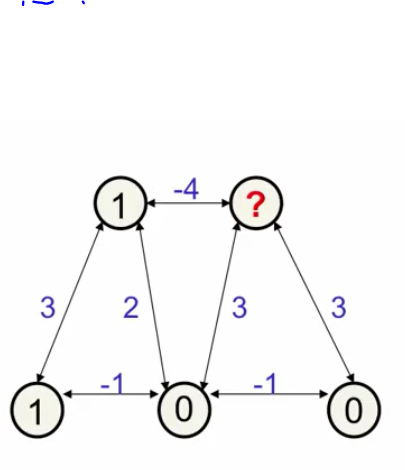
\includegraphics[scale=0.8]{sections/11/picked.png}
	\end{center}
	\begin{center}
		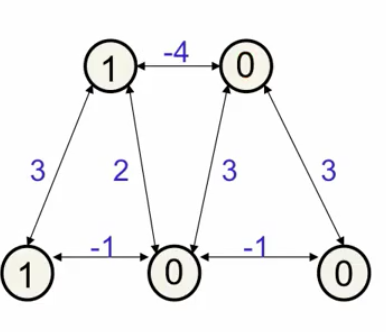
\includegraphics[scale=0.8]{sections/11/off.png}
	\end{center}

	$$-4(1)+3(0)+3(0)=-4<0\to \text{Turn off}$$
	\item Repeat for remaining units

	\subsubsection{A deeper energy minimum}
	\item The net has two triangles in which the three units mostly support each other
	\item Each triangle mostly hates the other triangle (-4 at the top)
	\item The triangle on the left differs from the one on the right by having a weight of 2 where the other one has a weight of 3
	\item So turning on the units in the triangle on the right gives the deepest minimum.
	\begin{center}
		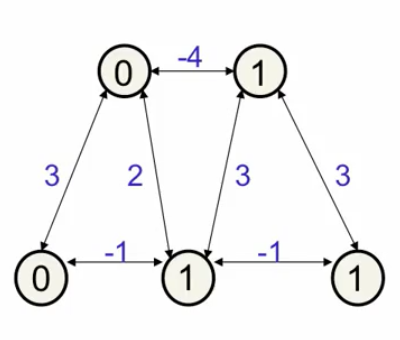
\includegraphics[scale=0.8]{sections/11/deep.png}
	\end{center}

	\subsubsection{Who do the decisions need to be sequential?}
	\item If units make simultaneous decisions the energy could go up
	\item With simultaneous parallel updating we can get oscillations
	\begin{itemize}
		\item Two units will continue to flip on and off
		\begin{center}
			\includgraphics[scale=0.9]{osc.png}
		\end{center}
		\item At the next parllel step, both units will turn on. This has very high energy, so then they will both turn off again.
	\end{itemize}

	\item If the updates occur in parallel but with random timing, the oscillations are usually destroyed
	
	\subsubsection{A neat way to make use of this type of computation}
	\item Hopfield proposed that memories could be energy minima of a neural net
	\begin{itemize}
		\item The binary threshold decision rule can then be used to ``clean up'' incomplete or corrupted memories
	\end{itemize}
	\item The idea of memories as energy minima was proposed by I.A. Richards in 1924 in ``Principles of Literary Criticism''
	\item Using energy minima to represent memories gives a content-adressable memory
	\begin{itemize}
		\item An item can be assessed by just knowing part of its content
		\item It is robust against hardware damage
		\item It's like reconstructing a dinosaur from a few bones
	\end{itemize}

	\subsubsection{Storing memories in a Hopfield net}
	\item If we use activities of 1 and -1, we can store a binary state vector by incrementing the weight between any two units by the product of their activities.
		$$\delta w_{ij} = s_i s_j$$
	\item This is a very simple rule that is not error-driven.That is both its strenght and its weakness. 
	\item We treat biases as weights from a permanently on unit
	\item With states of 0 and 1 the rule is slightly more complicated:
		$$\delta w_{ij} = 4(s_i - \frac{1}{2})(s_j - \frac{1}{2})$$
\end{itemize}

\section{Polymorphism}
	\subsection{Boltzmann machine learning}
\begin{itemize}
	\item Unsupervised learning problem
	\item We want the maximize the product of the probabilities that the Boltzmann machine assigns to the binary vectors in the training set
	\item Equivalent to maximizing the sum of the log probabilities that the Boltzmann machine assigns to the training vectors
	\item It is also equivalent to maximizing hte probability that we would obtain exactly the N training cases if we did the following:
	\begin{itemize}
		\item Let the network settle to its stationary distribution N different times with no external input
		\item Sample the visible vector once each time
	\end{itemize}

	\subsubsection{Why the learning could be difficult}
	\item Consider the chain of units:
	\begin{center}
		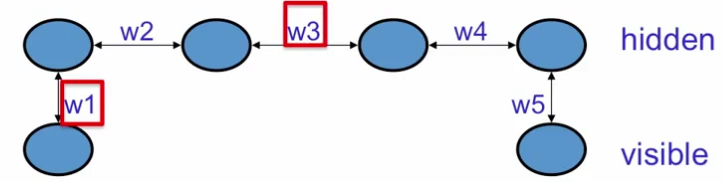
\includegraphics[scale=0.6]{sections/12/chain.png}
	\end{center}
	\item If the raining set consists of (1,0) and (0,1) we want the product of all the weights to be negative (So to know how to change w1 or w5 we must know w3)

	\item Everything that one weight needs to know about the other weights and the data is contained in the difference of two correlations:
	\begin{center}
		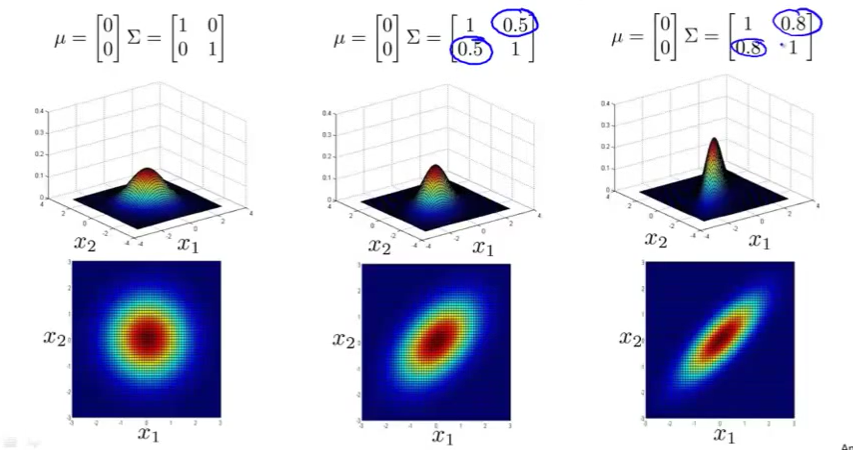
\includegraphics[scale=0.6]{sections/12/corr.png}
	\end{center}
		$$\delta w_{ij} \propto \langle s_i s_j \rangle_{data} - \langle s_i s_j \rangle_{model}$$

	\subsubsection{Why is the derivative so simple?}
	\item THe probability of a global configuration at thermal equilibrium is an exponential function of its energy
	\item So setting to equilibrium makes the log probability a linear function of the energy
	\item The energy is a linear fnuction of the weights and states, so:
		$$-\frac{\partial E}{\partial w_{ij}}=s_i s_j$$

	\item The process of settling to thermal equilibrium propagates information about the weights (We dontt need backprop)

	\subsubsection{Why do we need the negative phase?}
	\item Probability of a visible vector:
	\begin{center}
		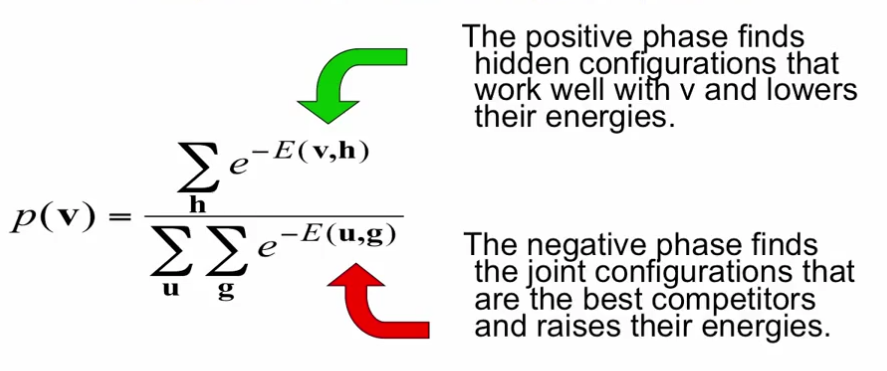
\includegraphics[scale=0.6]{sections/12/neg.png}
	\end{center}

	\subsubsection{An inefficient way to collect the statistics required for learning}
	\item \textbf{Positive phase}: clamp a data vector on the visible units and set the hidden units to random binary states
	\item Update the hidden units one at a time until the network reaches thermal equilibrium at a temperature of 1
	\item Once equilibrium, Sample $s_i s_j$ for every connected pair of units
	\item Repeat for al ldata vectors in the training set and average
	\item \textbf{Negative phase}: Set all the units to random states
	\item Update until equilibrium at temperature of 1
	\item Sample $s_i s_j$ for every connected pair of units
	\item Repeat many times and average to get good estimates
\end{itemize}

\section{Container ADTs}
	\subsection{The ups and downs of backpropagation}
\begin{itemize}
	\subsubsection{A brief history of backpropagation}
	\item The backpropagation algorithm for learning multiple layers of features was invented several times in the 70's and 80's:
	\begin{itemize}
		\item Bryson \& Ho (1969) linear
		\item Werbos (1974)
		\item Rumelhart et. al. in 1981
		\item Parker (1985)
		\item LeCun (1985)
		\item Rumelhart et.al. (1985)
	\end{itemize}

	\item Backpropagation clearly had great promise for learning multiple layers of non-linear feature detectors
	\item But by the late 1990's most serious researchers in machine learning had given up on it
	\begin{itemize}
		\item It was still widely used in psychological models and in practical pplications such as credit card fraud detection
	\end{itemize}

	\subsubsection{Why backpropagation failed}
	\item The popular explanation of why backpropagation failed in the 90's:
	\begin{itemize}
		\item It could not make good use of multiple hidden layers
		\item It did not work well in recurrent networks or deep auto-encoders
		\item Support vector machines worked better, required less expertise, produced repeatable results, and had a much better theory
	\end{itemize}

	\item The real reason it failed:
	\begin{itemize}
		\item Computers were thousands of times too slow
		\item Labeled datasets were hundreds of times too small
		\item Deep networks were too small and not initialized sensibly
	\end{itemize}

	\subsubsection{A spectrum of machine learning tasks}
	\item Theres a spectrum of tasks from the things people study in typical statistics to artificial intelligence
	\item Statistics end of the spectrum:
	\begin{itemize}
		\item Low-dimensional data (e.g., less than 100 dimensions)
		\item Lots of noise in the data
		\item Not much structure in the data. The structure can be captured by a fairly simple model
		\item The main problem is separating true structure from noise
		\begin{itemize}
			\item Not ideal for non-Bayesian neural nets. Try SVM or GP.
		\end{itemize}
	\end{itemize}

	\item Artificial intellience end of the spectrum:
	\begin{itemize}
		\item High-dimensional data (e.g., more than 100 dimensions)
		\item The noise is not the main problem
		\item There is a huge amount of structure in the data, but its too complicated to be represented by a simple model
		\item The main problem is figuring out a way to represent the complicated structure so that it can be learned
		\begin{itemize}
			\item Let backpropagation figure it out
		\end{itemize}
	\end{itemize}

	\subsubsection{Why Support Vector Machines were never a good bet for Artificial Intelligence tasks that need good representations}
	\item \textbf{View 1}: SVM's are just a clever reincarnation of Perceptrons
	\begin{itemize}
		\item They expand the input to a very large layer of non-linear non-adaptive features 
		\item They only have one layer of adaptive weights 
		\item They ahve a very efficient way of fitting the weights that control overfitting (max margin hyperplane)
	\end{itemize}
	\item \textbf{View 2}: SVM's are just a clever reincarnation of Perceptrons (different notion of features being used)
	\begin{itemize}
		\item They use each input vector in the training set to define a non-adaptive ``feature''
		\begin{itemize}
			\item How similar a test input is to a training case
		\end{itemize}
		\item They have a clever way of simultaneously doing feature selection and finding weights on the remaining features.
	\end{itemize}
\end{itemize}

\subsection{Belief Nets}
\begin{itemize}
	\item 
\end{itemize}

\section{Interfaces and Invariants}
	\subsection{Interfaces}
\begin{itemize}
	\item Question: How can you provide a class definition that carries no implementation details to the client programmer, yet still has interface information?
	\item Answer: Create an ``interface-only'' class as an abstract base class, from which an implementation can be derived.
	\item Interfaces have \textbf{no implementation} which makes it different from an abstract class, which may have partial implementation.
	\item This is done using pure virtual functions
	\item e.g., (Notice how all of the functions are pure virtual)
\begin{lstlisting}[style=C++]
class IntSet{
	// OVERVIEW: interface for a mutable set of ints
	// with bounded size

public:
	virtualvoid insert(intv) = 0;
	virtualvoid remove(intv) = 0;
	virtualboolquery(intv) const= 0;
	virtualintsize() const= 0;
};
\end{lstlisting}
	\item You \textbf{cannot} instantiate \lstinline[style=C++]{IntSet}, because there is no implementation
	\item You can create a pointer however
	\item e.g.,
\begin{lstlisting}[style=C++]
intmain() {
	IntSetUnsortedis;
	IntSet*is_ptr= &is; //pointer to implementation
	is_ptr->insert(7);
	is_ptr->insert(4);
	is_ptr->insert(7);
	is_ptr->insert(1);
	is_ptr->remove(4);
}
\end{lstlisting}
\end{itemize}

\subsection{Representation Invariant Details}
\begin{itemize}
	\item A \textit{representation invariant} must be true immediately before and immediately after any member function execution
	\item With two \textbf{exceptions} of course:
	\begin{itemize}
		\item \textbf{Constructors}: the constructor establishes the representation invariant, so the representation invariant only has to hold at the end
		\item \textbf{Destructors}: the representation invariant only has to hold at the beginning
	\end{itemize}
	\item You may find it helpful to create a \lstinline[style=C++]{check_invariant()} function to run tests on whether your functions maintain their representation.
\end{itemize}

\section{Memory Models}
	\subsection{Global variables}
\begin{itemize}
	\item Global variables are defined anywhere outside of a function definition
	\item Space is set aside for these variables before the program begins execution, and is reserved for them until the program completes
	\item This space is reserved at compile time
	\item e.g.,
\begin{lstlisting}[style=C++]
const int SIZE=10;	// Global variable
int main() {
	//...
}
\end{lstlisting}
\end{itemize}

\subsection{Local variables}
\begin{itemize}
	\item Local variables are any variable defined within a block
	\item This includes function arguments, which act as if they were defined in the outermost block of the function
	\item Space is set aside for these variables when the relevant block is entered, and is reserved for them until the block is exited
	\item This space is reserved at run time, but the size is known to the compiler
	\item e.g.,
\begin{lstlisting}[style=C++]
int sum(int *array, int size) {
	int sum=0; 	// Local variable, alongside array (the pointer!) and size
	//...
}
\end{lstlisting}
\end{itemize}

\subsection{Dynamic variables}
\begin{itemize}
	\item It is dynamic because:
	\begin{itemize}
		\item Size (or number) is determined at runtime
		\item When it will be created and destroyed is determined at runtime
	\end{itemize}
\end{itemize}

\subsubsection{new}
\begin{itemize}
	\item Create dynamic variables using new
\begin{lstlisting}[style=C++]
int main() {
	int *p = new int;
}
\end{lstlisting}
	\item This creates new space for an integer, and returns a pointer to that space, assigning it to \lstinline[style=C++]{p}
	\item The initial value is undefined
	\item Use initializer syntax to assign an initial value:
\begin{lstlisting}[style=C++]
int main() {
	int *p = new int(5);
}
\end{lstlisting}
\end{itemize}

\subsubsection{delete}
\begin{itemize}
	\item Destroy dynamic variables using \lstinline[style=C++]{delete}
\begin{lstlisting}[style=C++]
int *p= new int;
//do something with p
delete p;
delete p; //Error!
\end{lstlisting}
	\item Releases the claim on the space previously used by the \lstinline[style=C++]{int}
	\item You can only \lstinline[style=C++]{delete} a dynamic variable \textit{once}
\begin{lstlisting}[style=C++]
delete p;
delete p; //Error!
\end{lstlisting}
	\item Assigning NULL to deleted pointers prevents this issue:
\begin{lstlisting}[style=C++]
delete p; p=0;
delete p; // Ok
\end{lstlisting}
	\item Only objects that are created with \lstinline[style=C++]{new} can be destroyed by \lstinline[style=C++]{delete}
\end{itemize}

\subsubsection{Dynamic array}
\begin{itemize}
	\item e.g.,
\begin{lstlisting}
//ask user to enter integer size
int size = get_size_from_user();

int *p= new int[size];
//do something with p ...
delete[] p;
\end{lstlisting}
\end{itemize}

\subsection{Memory leaks}
\begin{itemize}
	\item Dynamic variables live until the programmer destroys them using \lstinline[style=C++]{delete}
	\item This is true even if you ``forge'' the pointer to the object.
\begin{lstlisting}[style=C++]
int main() {
	int *p1 = new int(1);
	int *p2 = new int(2);
	p1 = p2;
}
\end{lstlisting}
	\begin{center}
		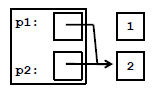
\includegraphics{sections/lec15/mem1.png}
	\end{center}
	\item This leaves us with an allocated dynamic object that wehave no means of reclaiming called a \textbf{memory leak}
\end{itemize}

\subsection{The heap}
\begin{itemize}
	\item The space for objects created via \lstinline[style=C++]{new} comes from a location in memory called the heap.
	\item A running program has an ``address space'', a collection of memory locations that are accessible to it
	\begin{center}
		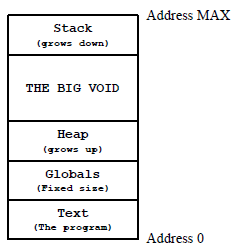
\includegraphics{sections/lec15/mem2.png}
	\end{center}
	\item \textbf{Text segment}: the code comprising a compiled program goes in the text segment.
	\item \textbf{Globals}: the compiler allocates space for any global variables
	\item \textbf{Heap}: when things are allocated via \lstinline[style=C++]{new}, they come from the heap
	\item \textbf{Stack}: stack frames are created on the stack, which grows downward
	\item \textbf{Big void}: since we don't know howbig either of these will get, we keep a big hole in between the two
	\item \textbf{Little void}: the first thousand addresses starting at zero are reserved for accidental use of as an \lstinline[style=C++]{int} as a pointer, resulting in a SEGFAULT.
\end{itemize}

\subsection{Global vs. Local vs. Dynamic}
\begin{center}
\begin{tabular}{l|l|l|l}
	& Global & Local & Dynamic \\
	\hline
	Where in code? & Outside function & Inside function (block) or args & Anywhere you use new \\
	When created? & Beginning of program & Beginning of function (block) & You call new \\
	When destroyed? & End of program & End of function & You call delete \\
	Size? & static & static & dynamic \\
	Location? & Globals & Stack & Heap \\
\end{tabular}
\end{center}
\begin{itemize}
	\item See example from lecture slides.
\end{itemize}

\subsection{Classes and dynamic memory}
\begin{itemize}
	\item When you create instances of classes, their constructors are called, just as if it were created the ``normal'' way.
\begin{lstlisting}[style=C++]
IntSet *isp = new IntSet;
\end{lstlisting}
	\begin{enumerate}
		\item Allocate enough space on the heap to hold an \lstinline[style=C++]{IntSet}
		\item Call the constructor \lstinline[style=C++]{IntSet::IntSet()} on this new object
	\end{enumerate}
\end{itemize}

\section{Copying Arrays}
	\subsection{Default Argument}
\begin{itemize}
	\item One way to solve this problem of duplicate definitions is to use something called a \textit{default argument}
	\item \textbf{Default argument}: make an argument optional by specifying the value to be assigned when not specified (default)
\begin{lstlisting}[style=C++]
IntSet(int capacity = 0);
\end{lstlisting}
\end{itemize}

\subsection{Destructor}
\begin{itemize}
	\item Problem: what happens if we have a local \lstinline[style=C++]{IntSet} inside of a function and the function returns?
\begin{lstlisting}[style=C++]
void foo() {
	IntSet is(3);
}  // foo returns

int main() {
	foo();
}
\end{lstlisting}
	\item Array is stored on the heap, and only the pointer will be destroyed.
	\item To solve this memory leak, we have to arrange to de-allocate the integer array whenever the ``enclosing'' IntSetis destroyed.
	\item We do this with a \textbf{destructor}, the opposite of a constructor
	\item A destructor also has the same name as the class, preceded with a tilde
	\item e.g.,
\begin{lstlisting}[style=C++]
class IntSet{
public:
	//...

	//EFFECTS: destroys this IntSet
	~IntSet();

	//...
};

IntSet::~IntSet() {
	delete[] elts;
}
\end{lstlisting}
	\item Destructors run automatically when an object is destroyed
	\item When does the destructor run?
	\begin{itemize}
		\item Local: out of scope
		\item Global: program end
		\item Dynamic: \textbf{when it is deletec}
	\end{itemize}
\end{itemize}

\subsection{Copy Constructor}
\begin{itemize}
	\item In our original \lstinline[style=C++]{IntSet} when a copy is currently performed the pointer to the array of the original set is copied, so both sets will have pointers point to one array. 
	\item The copy constructor has two tasks
	\begin{enumerate}
		\item Initialize the member variables
		\item \textbf{Copy everything} from the other \lstinline[style=C++]{IntSet}
	\end{enumerate}
	\item e.g.,
\begin{lstlisting}[style=C++]
IntSet::IntSet(constIntSet&other) {
	//1. Initialize member variables
	elts= new int[other.elts_capacity];
	elts_size= other.elts_size;
	elts_capacity= other.elts_capacity;

	//2. Copy everything from the other IntSet
	for (inti= 0; i< other.elts_size; ++i)
		elts[i] = other.elts[i];
}
\end{lstlisting}
	\item The copy constructor we've written follows pointers and copiesthe things they point to, rather than just copying the pointers
	\item This is called a \textbf{deep copy}, as opposed to the default behavior which called a \textbf{shallow copy}
\end{itemize}

\subsection{Destructors and polymorphism}
\begin{itemize}
	\item When you create a object, all the constructors run, starting with the base class
	\item Now, let's see what happens when we mix destructors with polymorphism
	\item e.g.,
\begin{lstlisting}[style=C++]
class Animal {
	virtual void talk() {}
	virtual ~Animal {}
};

class Chicken : public Animal {
public:
	virtual void talk()
		{ cout<< "cluck\n"; }
	virtual ~Chicken {}
};

class Horse : public Animal {
public:
	virtual void talk()
		{ cout<< “neigh\n"; }
};
\end{lstlisting}
	\item When running the following code:
\begin{lstlisting}[style=C++]
Animal *a = ask_user(); //input: “Chicken”
// do something with a
delete a; a=0;
\end{lstlisting}
	\item Since dtoris virtual, correct dtors(\lstinline[style=C++]{~Chicken()}, then \lstinline[style=C++]{~Animal()} ) are selected at runtime.
	\item Destructors run from child class towards parent class!
\end{itemize}

\section{Deep Copies and Resizing}
	\subsection{Problems with assignment ``=''}
\begin{itemize}
	\item Same issue with copy constructor, it does a shallow copy
	\item \textbf{Operator overloading} lets us customize what happens when we use a built-in symbol.
\begin{lstlisting}[style=C++]
class IntSet{
	// data elements
	// ...

public:
	// Constructors
	// EFFECTS: assignment operator does a deep copy
	IntSet &operator= (const IntSet &rhs);
	//...
};
\end{lstlisting}
	\item Like the copy constructor, the assignment operator takes a reference to a const instance to copy from
	\item However, it also returnsa reference to the copied-to object.
	\item This return value allows for a chained assignmentlike this: \lstinline[style=C++]{is3 = is2 = is1; }
\end{itemize}

\subsection{Understanding this}
\begin{itemize}
	\item We need to return a reference to the current \lstinline[style=C++]{IntSet} so that chaining works
	\item Every member function has a ``secret'' variable called \lstinline[style=C++]{this}
	\begin{itemize}
		\item \lstinline[style=C++]{this} is a pointer to the current instance of the class
		\item Here, we use \lstinline[style=C++]{*this} because the reutrn type isa reference
	\end{itemize}
	\item Think of \lstinline[style=C++]{this} as a local variable which points to the current instance
	\begin{center}
		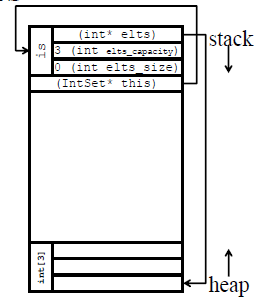
\includegraphics{sections/lec17/this.png}
	\end{center}
\end{itemize}

\subsection{The Rule of the Big Three}
\begin{itemize}
	\item If you have any dynamically allocated storage in a class, you must provide:
	\begin{enumerate}
		\item A destructor
		\item A copy constructor
		\item An overloaded assignment operator
	\end{enumerate}
\end{itemize}

\section{Linked Lists}
	\begin{itemize}
	\item A linked structure is one with a series of zero or more pieces of data, connected by pointers from one to another
	\begin{center}
		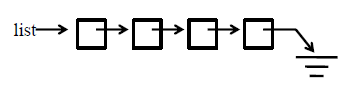
\includegraphics{sections/lec18/ll.png}
	\end{center}
	\item A list is another example of a container ADT
\end{itemize}

\subsection{List nodes}
\begin{itemize}
	\item We need to pick a concrete representation that stores a list as a dynamically created list of ``nodes''
\begin{lstlisting}[style=C++]
structNode {
	Node *next;
	int datum;
};
\end{lstlisting}
	\item Invariant:
	\begin{itemize}
		\item the datum field holds the integer datum of an element in the list
		\item Invariant: the next field points to the next Nodein the list, or 0 (AKA NULL) if no such Node exists
	\end{itemize}
	\item Resulting in the list's concrete implementation in the form of:
	\begin{center}
		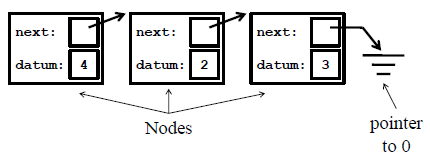
\includegraphics{sections/lec18/l1.png}
	\end{center}
\begin{lstlisting}[style=C++]
class IntList{
	//...
private:
	struct Node {
		Node *next;
		int datum;
	};
	Node *first;
};
\end{lstlisting}
	\item Representation invariant: \lstinline[style=C++]{first} points to the first node in the sequence of nodes representing this \lstinline[style=C++]{IntList}, or 0 if the list is empty
\end{itemize}

\subsection{Insert}
\begin{itemize}
	\item 
\begin{lstlisting}[style=C++]
void IntList::insertFront(int i) {
	Node *np= new Node;
	np->datum = i;
	np->next = first;
	first = np;
}
\end{lstlisting}
\begin{center}
	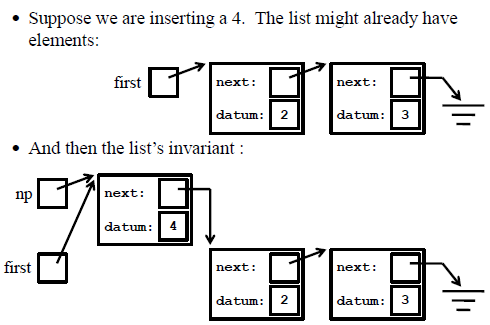
\includegraphics{sections/lec18/front.png}
\end{center}
\end{itemize}

\subsection{Implementing removeFront()}
\begin{itemize}
	\item If we are removing this first node, we must delete it to avoid a memory leak
	\item Unfortunately, we can't delete it before advancing the first pointer
\begin{lstlisting}[style=C++]
int IntList::removeFront() {
	assert(!isEmpty());
	Node *victim = first;
	first = first->next;
	int result = victim->datum;
	delete victim; victim=0;
	return result;
}	
\end{lstlisting}
\end{itemize}

\subsection{Implementing insertBack()}
\begin{itemize}
	\item Adding a member variable to point to the last item in a list, allows for trivial insert back
\begin{lstlisting}[style=C++]
void IntList::insertBack(inti) {
	Node *np= new Node;
	np->datum = i;
	np->next = 0;
	if (isEmpty()) {
		first = last = np;
	} else {
		last->next = np;
		last = np;
	}
}
\end{lstlisting}
\begin{center}
	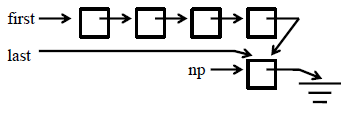
\includegraphics{sections/lec18/back.png}
\end{center}
	\item Removing from back is expensive because you must find the previous to last node: $\O{n}$
\end{itemize}

\subsection{Singly linked vs. doubly linked lists}
\begin{itemize}
	\item To make removal from the end efficient, as well, we have to have a doubly-linked list, so we can go forward and backward.
	\item In our new representation, a node is:
\begin{lstlisting}[style=C++]
structNode {
	Node *next;
	Node *prev;
	int datum;
}
\end{lstlisting}
	\item e.g., $[2, 3]$
\begin{center}
	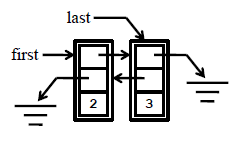
\includegraphics{sections/lec18/dl.png}
\end{center}
\end{itemize}

\section{Templated Containers}
	\subsection{Introduction}
\begin{itemize}
	\item Abstract Data Types like \lstinline[style=C++]{IntSet} and \lstinline[style=C++]{IntList} are often called \textbf{containers} or container classes, since their purpose is to contain other objects
	\item Today, we will use the C++ \lstinline[style=C++]{template} mechanism to reuse the same container code for any type
	\item To see how templates might be useful, consider the following fragments defining a list-of-intand a list-of-char:
\begin{lstlisting}[style=C++]
// Int 
class List {
public:
	void insertFront(int v);
	int removeFront();
	//...
private:
	struct Node { 
		Node *next;
		int datum;
	};
	Node *first;
};

// Char 
class List {
public:
	void insertFront(char v);
	char removeFront();
	//...
private:
	struct Node { 
		Node *next;
		int datum;
	};
	char *first;
};
\end{lstlisting}
	\item It's like someone took the list-of-int definition and replaced each instance of \lstinline[style=C++]{int} with an instance of \lstinline[style=C++]{char}.
\end{itemize}

\subsection{Templates}
\begin{itemize}
	\item The intuition behind templates is that they are code with the ``type name'' left as a (compile-time) constant.
	\item The parameter is a type, not a variable.
	\item To start, you first need to declare that something will be a template:
\begin{lstlisting}[style=C++]
template <typename T>
class List {
	// ...
};
\end{lstlisting}
	\item \lstinline[style=C++]{T} stands for ``the name of the type contained by this \lstinline[style=C++]{List}''
	\item Alternate notation:
\begin{lstlisting}[style=C++]
template <class T>
class List {
	// ...
};
\end{lstlisting}
	\item e.g.,
\begin{lstlisting}[style=C++]
template <typename T>
class List {
public:
	// methods

	// constructors/destructor

private:
	struct Node {
		Node *next;
		T datum;
	};
	//...
};
\end{lstlisting}
\end{itemize}

\subsection{Templated Methods}
\begin{itemize}
	\item All that is left is to define each of the method bodies.
	\item Each body must also be declared as a templated method and we do that in much the same way as we do for the class definition
	\item Each function begins with the template declaration: \lstinline[style=C++]{template <typename T>}
	\item And each method name must in the \lstinline[style=C++]{List<T>} scope:
\begin{lstlisting}[style=C++]
template <typename T>
void List<T>::insertFront(Ti) {
	Node *np= new Node;
	np->datum = i;
	np->next = first;
	first = np;
}
\end{lstlisting}
\end{itemize}

\subsection{Using Templated Containers}
\begin{itemize}
	\item To use the templated container, you specify the type \lstinline[style=C++]{T} when creating the container object.
\begin{lstlisting}[style=C++]
// Create a list of integers on the stack
List<int> li;
li.insertFront(42);

// Create a list of integers on the heap
List<int> *lip = new List<int>;
lip->insertFront(42);
\end{lstlisting}
	\item All templated codes goes in the header file: both the declaration and definition
\end{itemize}

\subsection{Containers of large values}
\begin{itemize}
	\item Copying elements by value is fine for types with small representations, for example, built-in types like \lstinline[style=C++]{int}
	\item This is nottrue for larger types –any nontrivial structor class would be expensive to pass by value, because you'll spend all of your time copying
	\item e.g.,
\begin{lstlisting}[style=C++]
class Gorilla {
	// OVERVIEW: a big, expensive class
	// lots of member data ...
};\end{lstlisting}
	\item Two options:
	\begin{itemize}
		\item Pass-by-pointer (results in container of pointers)
		\item Pass-by-reference (only fixes parameter copy issues)
	\end{itemize}
\end{itemize}

\subsubsection{Container of pointers}
\begin{itemize}
	\item The good news: \lstinline[style=C++]{Gorilla} is passed by pointer, no copies!
	\item The bad news: containers-of-pointers are subject to two broad kinds of potential bugs:
	\begin{enumerate}
		\item Using an object after it has been deleted
\begin{lstlisting}[style=C++]
List<Gorilla*> zoo;
Gorilla *colo= new Gorilla;
zoo.insertFront(colo);
// ...
delete colo; // bad!
// ...
Gorilla *g = zoo.removeFront();//g already deleted!
\end{lstlisting}
		\item Leaving an object orphaned by neverdeleting it
	\end{enumerate}
\end{itemize}

\subsection{Pattern of use for container-of-ptr}
\begin{enumerate}
	\item \textbf{Existence}: Allocate an object before inserting it into any container.
\begin{lstlisting}[style=C++]
// OK
List<Gorilla*> zoo;
Gorilla *colo= new Gorilla;
zoo.insertFront(colo);

// better
List<Gorilla*> zoo;
zoo.insertFront(new Gorilla);
\end{lstlisting}
	\item \textbf{Ownership}: Once it is inserted, do not modify it until it is removed.
\begin{lstlisting}[style=C++]
List<Gorilla*> zoo;
Gorilla *colo= new Gorilla;
zoo.insertFront(colo);
colo->set_name("Bill"); // bad! - could mess up a container's representation invariant

// Good:
Gorilla *g = zoo.removeFront(); //remove
g->set_name("Bill"); //change
zoo.insertFront(g); //replace
\end{lstlisting}
	\item \textbf{Conservation}: Once it is removed, it must either be deallocatedor inserted into some container. Don’t forget to delete at the end!
\begin{lstlisting}[style=C++]
// bad example
List<Gorilla*> zoo;
zoo.insertFront(new Gorilla);
zoo.removeFront(); //bad! memory leak!

// good example
List<Gorilla*> zoo;
zoo.insertFront(new Gorilla);
deletezoo.removeFront(); // fixed
\end{lstlisting}
\end{enumerate}

\subsection{Deleting a shared object}
\begin{itemize}
	\item How to delete objects that occur on multiple containers?
	\item One solution:
	\begin{itemize}
		\item Remove object from allcontainers before freeing up the object.
	\end{itemize}
\end{itemize}

\section{Iterators}
	\begin{itemize}
	\item An iterator allows you to traverse a container
	\item We’ve seen something like this before with arrays
\begin{lstlisting}[style=C++]
int a[SIZE]; // fill a
for (int i=0; i< SIZE; ++i)
	cout<< a[i] << endl;
\end{lstlisting}
	\item How would you do this for a linked list, like our \lstinline[style=C++]{List} type?
	\item In the end, our iterator will work a lot like using a pointer to traverse an array
\end{itemize}

\subsection{Iterator functions}
\begin{enumerate}
	\item \textbf{Create}: an iterator with a constructor
	\item \textbf{Get}: the \lstinline[style=C++]{T} at the iterator’s current position
	\item \textbf{Move}: the iterator to the next position
	\item \textbf{Compare}: two iterators
\end{enumerate}
\begin{lstlisting}[style=C++]
<template T>
class Iterator {
	Node* node_ptr;
public:
	Iterator(); 							// Create
	T& operator* () const; 					// Get
	Iterator& operator++ (); 				// Move
	bool operator!= (Iterator rhs) const;	// Compare
};
\end{lstlisting}

\subsection{Friends}
\begin{itemize}
	\item Our list also needs to functions \lstinline[style=C++]{begin(), end()} 
	\item \lstinline[style=C++]{begin()}: returns an iterator object pointing to first list position
	\item \lstinline[style=C++]{end()}: returns a default iterator object ``past the end'' position
	\item Our \lstinline[style=C++]{Iterator} needs access to the internal workings of the \lstinline[style=C++]{List} in order to perform these functions
	\item We can solve this by making \lstinline[style=C++]{Iterator} a \textbf{friend} of \lstinline[style=C++]{List}
	\item Friendship is \textbf{given}, not taken
	\item The class declares which classes are its friends
	\item e.g.,
\begin{lstlisting}[style=C++]
class List {
	// ...
	class Iterator {
		// ...
		friend class List;
	};
};
\end{lstlisting}
\end{itemize}

\subsection{Using iterators}
\begin{itemize}
	\item With these functionalities we can now use an iterator to traverse a list:
\begin{lstlisting}[style=C++]
List<int> l;
l.insertFront( 3 );
l.insertFront( 2 );
l.insertFront( 1 );

for (List<int>::Iterator i=l.begin(); i!= l.end(); ++i) {
	cout<< *i<< " ";
}

cout<< endl;
\end{lstlisting}
	\item We have successfully created a function abstraction to access a container
\end{itemize}

\subsection{Iterator invalidation}
\begin{itemize}
	\item Once an iterator is created, if the underlying container is modified, the iterator may become invalid.
	\item If the iterator is invalidated, its behavior is undefined, much like an invalid pointer.
	\item The intuition behind this is that the iterator depends on the representation of the container – if that changes, the iterator is likely to miss an element or return an element that no longer exists.
	\item e.g., (BAD)
\begin{lstlisting}[style=C++]
List<int> l;
l.insertFront( 1 );
List<int>::Iterator i=l.begin();
++i; ++i; // oops, went off the end!
\end{lstlisting}
	\item It’s your responsibility to keep your Iterator within the bounds of the container
\end{itemize}

\subsection{Putting it all together}
\begin{lstlisting}[style=C++]
List<Gorilla*> zoo;
zoo.insertFront(new Gorilla("Colo"));
zoo.insertFront(new Gorilla("Koko"));

for (List<Gorilla*>::Iterator i=zoo.begin(); i!= zoo.end(); ++i)
	cout<< (**i).get_name() << endl;

for (List<Gorilla*>::Iterator i=zoo.begin(); i!= zoo.end(); ++i) {
	delete *i; *i=0;
}

cout<< endl;
\end{lstlisting}

\section{Functors}
	\subsection{First-class Objects}
\begin{itemize}
	\item For any entity in a programming language, we say that the entity is \textbf{first-class} if you can do all four of these things:
	\begin{enumerate}
		\item Create them
		\item Destroy them
		\item Pass them as arguments
		\item Return them as values
	\end{enumerate}
	\item Unlike values, types and functions are notfirst class objects in C++; but, they can sometimes come close.
	\item The \textbf{template mechanism} allows us to pass types as arguments
	\item The \textbf{function pointer mechanism} allows us to pass functions as arguments and return them as results
\end{itemize}

\subsection{Motivation}
\begin{itemize}
	\item \lstinline[style=C++]{any_even, any_odd} are both very similar functions.
	\item We would like a function that is generic, and could perform a more general form of this operation
	\item The generic function signature would like like this:
\begin{lstlisting}[style=C++]
bool any_of(const List<int> &l, bool (*pred)(int));
\end{lstlisting}
\end{itemize}

\subsection{Using function pointers}
\begin{itemize}
	\item \lstinline[style=C++]{pred} is a pointer to a function that takes a single integer argument, returning a boolean result
	\item A \textbf{predicate} is used to control an algorithm
	\item The generic implementation is:
\begin{lstlisting}[style=C++]
bool any_of(const List<int> &l, bool (*pred)(int)) {
	for(List<int>::Iterator i=l.begin(); i!=l.end(); ++i)
		if (pred(*i)) return true;

	//reached end without finding elt
	return false;
}
\end{lstlisting}
	\item We can get the odd elements, by using the appropriate predicate:
\begin{lstlisting}[style=C++]
bool isOdd(intn) {
	return (n%2);
}

List<int> l;
// fill l ...
bool contains_odd= any_of(l, isOdd);
\end{lstlisting}
\end{itemize}

\subsection{Functors}
\begin{itemize}
	\item We can redefine the paranthesis operator () and use a class as a function
	\item However, unlike functions with function pointers, objects can have per-object state, which allows us to specialize on a per-object basis.
	\item e.g.,
\begin{lstlisting}[style=C++]
class GreaterN{
	int limit;
public:
	GreaterN(int limit_in) : limit(limit_in) {}
	bool operator() (int n) {
		return n > limit;
	}
};
\end{lstlisting}
	\item We can use this class to ``generate'' specialized functors:
\begin{lstlisting}[style=C++]
GreaterNg2(2);
GreaterNg6(6);
cout<< g2(4) << endl;
cout<< g6(4) << endl;
\end{lstlisting}
	\item Another use for functors: \textbf{Comparison}: used to define order, takes two elements of the same type and ouputs a \lstinline[style=C++]{bool}
\end{itemize}

\section{Exceptions}
	\subsection{Detecting errors at runtime}
\begin{itemize}
	\item We want a means of recognizing and handling unusual conditions in your program at runtime, not just at compile time.
	\item A REQUIRES clause is just comments and cannot enforce the specification. Therefore, it is easy to pass parameters that violate the specification.
\end{itemize}

\subsection{Exceptions}
\begin{itemize}
	\item \textbf{Exceptions} let us detect an error in one part of the program and correct it in a different part of the program
	\item When an exception occurs, control transfers from normal-case code to the error handling code
	\item This error handling code then tries to correct the problem
	\begin{center}
		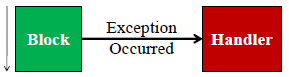
\includegraphics{sections/lec22/h.png}
	\end{center}
	\item When an exception occurs, it propagates from a function to its caller until it reaches a handler
	\item This is called \textbf{exception propagation}, and it happens automatically
\end{itemize}

\subsection{Exception Handling in C++}
\begin{itemize}
	\item When code detects an error, it uses a \lstinline[style=C++]{throw} statement
	\item Code that might cause an error goes in a \lstinline[style=C++]{try} block
	\item Code that corrects an error goes in a \lstinline[style=C++]{catch} block
	\item If the exception is successfully handled in the catch block, execution continues normally with the first statement following the catch block
	\item Otherwise, the exception is propagated to the enclosing block or to the caller if there is no enclosing block
	\item If an exception is propagated to the caller of \lstinline[style=C++]{main()}, the program exits
	\item When code detects an error, it uses a \lstinline[style=C++]{throw} statement
	\item When we throw an exception, we specify a value for the exception type in a throw statement
	\item e.g.,
\begin{lstlisting}[style=C++]
int n = 0; throw n;
char c = 'e'; throw c;
\end{lstlisting}
\end{itemize}

\subsection{Terminology}
\begin{itemize}
	\item Throw exception == raise exception
	\item Catch block == exception handler
\end{itemize}

\subsection{Exception Example}
\begin{itemize}
	\item Code that might cause an error goes in a \lstinline[style=C++]{try} block:
\begin{lstlisting}[style=C++]
int main() {
	string f; //function
	double n; //number
	
	while (cin>> f >> n) {
		try {
			if (f == "factorial") {
				cout<< factorial(n) << endl;
			}
		}catch(int i){
			cout << "try again" << endl;
		}
	}
}
\end{lstlisting}
	\item Code that corrects an error goes in a \lstinline[style=C++]{catch} block
	\item A \lstinline[style=C++]{catch} block goes directly after a \lstinline[style=C++]{try} block
	\item A \lstinline[style=C++]{catch} block matches the type from a \lstinline[style=C++]{throw} statement
\begin{lstlisting}[style=bash]
./a.out
factorial 5
120 
factorial -5
try again
\end{lstlisting}
	\item When an exception is not caught by a catch block, it propagates all the way to the caller of \lstinline[style=C++]{main}, and the program exits
\begin{lstlisting}[style=bash]
./a.out
combination -5 4
\item terminate called after thrown an instance of 'int'
Aborted (core dumped)
\end{lstlisting}
\end{itemize}

\subsection{Type discrimination}
\begin{itemize}
	\item A \lstinline[style=C++]{try} block can have multiple \lstinline[style=C++]{catch} blocks to handle different exception types
\begin{lstlisting}[style=C++]
try {
	if (foo) throw 4;
	// some statements go here
	if (bar) throw 2.0;
	// more statements go here
	if (baz) throw ‘a’;
}
catch (intn) { }
catch (double d) { }
catch (char c) { }
catch (...) { }
\end{lstlisting}
	\item The last handler is a \textbf{default handler}, which matches any exception type. It can be used as a ``catch-all'' in case no other catch block matches.
\end{itemize}

\subsection{Exception types}
\begin{itemize}
	\item Code often uses custom types to describe errors:
	\item e.g.,
\begin{lstlisting}[style=C++]
class NegativeError{};
class InputError{};
\end{lstlisting}
	\item We use the class mechanism to declare custom types
	\item When an error is detected, create a \lstinline[style=C++]{NegativeError} object and \lstinline[style=C++]{throw} it:
\begin{lstlisting}[style=C++]
//EFFECTS: returns n!, throws NegativeErrorfor n<0
int factorial (int n) {
	if (n<0) throw NegativeError();
	int result = 1;
	while (n > 0) {
		result *= n;
		n -= 1;
	}
	return result;
}

int main() {
	//...
	while (cin >> f >> n) {
		try {
			//...
		} catch (NegativeError){
			cout<< "try a positive number" << endl;
		} catch (...) {
			cout<< "try again" <<endl;
		}
	}
}
\end{lstlisting}
	\item See examples from lecture slides.
\end{itemize}

\end{document}